\documentclass{article}
\usepackage{tikz}
\usetikzlibrary{arrows.meta}

\begin{document}

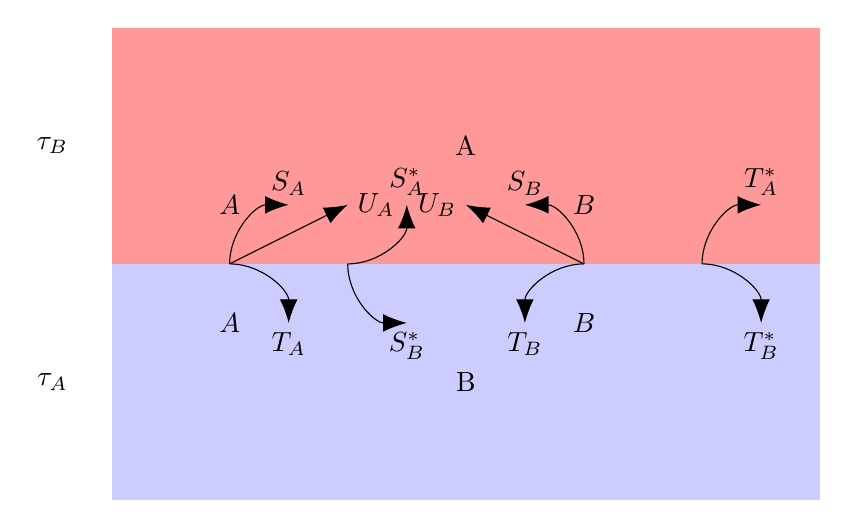
\begin{tikzpicture}[scale=1.5]
    % Define colors
    \definecolor{layerA}{RGB}{204,204,255} % Light blue
    \definecolor{layerB}{RGB}{255,153,153} % Light red

    % Draw the layers
    \fill[layerA] (0,0) rectangle (6,2);
    \fill[layerB] (0,2) rectangle (6,4);

    % Labels for the layers
    \node at (3,3) {A};
    \node at (3,1) {B};

    % Optical depth labels
    \node at (-0.5,1) {$\tau_A$};
    \node at (-0.5,3) {$\tau_B$};

    % Flux arrows
    \draw[-{Latex[length=3mm]}] (1,2) -- (2,2.5) node[right] {$U_A$};
    \draw[-{Latex[length=3mm]}] (4,2) -- (3,2.5) node[left] {$U_B$};

    % Scattering arrows
    \draw[-{Latex[length=3mm]}, bend left=45] (1,2) to (1.5,2.5) node[above] {$S_A$};
    \draw[-{Latex[length=3mm]}, bend right=45] (4,2) to (3.5,2.5) node[above] {$S_B$};

    % Transmission arrows
    \draw[-{Latex[length=3mm]}, bend left=45] (1,2) to (1.5,1.5) node[below] {$T_A$};
    \draw[-{Latex[length=3mm]}, bend right=45] (4,2) to (3.5,1.5) node[below] {$T_B$};

    % Starred transmission arrows
    \draw[-{Latex[length=3mm]}, bend left=45] (5,2) to (5.5,2.5) node[above] {$T_A^*$};
    \draw[-{Latex[length=3mm]}, bend right=45] (2,2) to (2.5,2.5) node[above] {$S_A^*$};

    % Starred scattering arrows
    \draw[-{Latex[length=3mm]}, bend left=45] (5,2) to (5.5,1.5) node[below] {$T_B^*$};
    \draw[-{Latex[length=3mm]}, bend right=45] (2,2) to (2.5,1.5) node[below] {$S_B^*$};

    % Layer labels
    \node at (1,2.5) {$A$};
    \node at (4,2.5) {$B$};
    \node at (1,1.5) {$A$};
    \node at (4,1.5) {$B$};
\end{tikzpicture}

\end{document}